\documentclass[tikz,border=5pt]{standalone}

\usepackage{graphicx}
\usepackage{comment}
\usepackage{tikz}
\usetikzlibrary{positioning}

\usepackage[scaled]{helvet}
\renewcommand{\familydefault}{\sfdefault}


\begin{document}
\begin{tikzpicture}[
  node distance = 1cm and 1.5cm,
  font=\sffamily,
  every node/.style={inner sep=0, outer sep=0}
]


\begin{comment}


# Making plots
python3 CounterfactualModel_VIZ_Components_Fig2.py 2 0 10.0 180 1000 UNIFORM STEEPPERIODIC 5
python3 RunSynthetic_FreePrior_CosineLoss_OnSim_VIZ_OnlyModel_OtherNoiseLevels_Fig2.py 2 0 10.0 180 SimulateSynthetic_Parameterized_OtherNoiseLevels_Grid_VarySize.py_180_2_5_N1000_UNIFORM_STEEPPERIODIC.txt
python3 RunSynthetic_FreePrior_CosineLoss_OnSim_VIZ_OnlyModel_OtherNoiseLevels_Fig2.py 2 0 10.0 180 SimulateSynthetic_Parameterized_OtherNoiseLevels_Grid_VarySize.py_180_2_5_N5000_UNIFORM_STEEPPERIODIC.txt
python3 RunSynthetic_FreePrior_CosineLoss_OnSim_VIZ_OnlyModel_OtherNoiseLevels_Fig2.py 2 0 10.0 180 SimulateSynthetic_Parameterized_OtherNoiseLevels_Grid_VarySize.py_180_2_5_N10000_UNIFORM_STEEPPERIODIC.txt
python3 RunSynthetic_FreePrior_CosineLoss_OnSim_VIZ_OnlyModel_OtherNoiseLevels_Fig2.py 2 0 10.0 180 SimulateSynthetic_Parameterized_OtherNoiseLevels_Grid_VarySize.py_180_2_5_N40000_UNIFORM_STEEPPERIODIC.txt
\end{comment}


%--- Top row: Ground truth
\node (plot-gt) {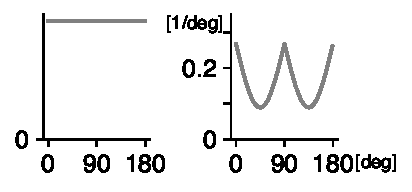
\includegraphics[width=0.45\textwidth]{figures/CounterfactualModel_VIZ_Components_Fig2.py_5_UNIFORM_STEEPPERIODIC_2_0_10.0_180.pdf}};
\node[above=0.1cm of plot-gt, anchor=center] (temp0) {};
\node[left=1.3cm of temp0, anchor=center] (prior-gt) {\large prior};
\node[right=1.9cm of prior-gt, anchor=center] (resources-gt) {\large resources};
\node[right=0.1cm of plot-gt.east, above=0.5cm of plot-gt.east, anchor=west] (gtlabel) {\large Ground truth};
\node[rotate=90, right=0.1cm of plot-gt.west, xshift=-0.3cm](prob-label){probability};
\node[above=0.2cm of temp0, anchor=center] (temp0-1) {};
\node[left=2.8cm of temp0-1, anchor=center](prob-label-a){\Large a};

%--- Second row: N=1000 (left), N=5000 (right)
\node[below=0.8cm of plot-gt.south, anchor=north] (label-1000) {\large N=1,000};
\node[below=0.4cm of label-1000, anchor=center] (temp1) {};
\node[left=1.3cm of temp1, anchor=center] (prior-1000) {\large prior};
\node[right=2.1cm of prior-1000, anchor=center] (resources-1000) {\large resources};
\node[below=0.5cm of label-1000, anchor=north, xshift=-0.1cm] (plot-1000)
  {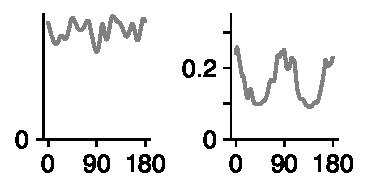
\includegraphics[width=0.4\textwidth]{figures/RunSynthetic_FreePrior_CosineLoss_OnSim_VIZ_OnlyModel_OtherNoiseLevels_Fig2.py_SimulateSynthetic_Parameterized_OtherNoiseLevels_Grid_VarySize.py_180_2_5_N1000_UNIFORM_STEEPPERIODIC.txt_2_0_10.0_180.pdf}};
\node[rotate=90, right=0.1cm of plot-1000.west, xshift=-0.4cm, yshift=-0.1cm](prob-label-1000){probability};
\node[above=0.2cm of temp1, anchor=center] (temp1-1) {};
\node[left=2.8cm of temp1-1, anchor=center](prob-label-b){\Large b};

\node[right=4cm of label-1000.east, anchor=center] (label-5000) {\large N=5,000};
\node[below=0.4cm of label-5000, anchor=center] (temp2) {};
\node[left=1.3cm of temp2, anchor=center] (prior-5000) {\large prior};
\node[right=2.1cm of prior-5000, anchor=center] (resources-5000) {\large resources};
\node[below=0.5cm of label-5000, anchor=north, xshift=-0.1cm] (plot-5000)
  {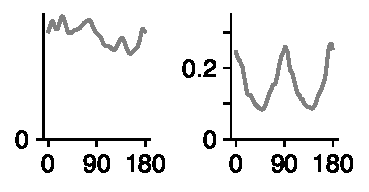
\includegraphics[width=0.4\textwidth]{figures/RunSynthetic_FreePrior_CosineLoss_OnSim_VIZ_OnlyModel_OtherNoiseLevels_Fig2.py_SimulateSynthetic_Parameterized_OtherNoiseLevels_Grid_VarySize.py_180_2_5_N5000_UNIFORM_STEEPPERIODIC.txt_2_0_10.0_180.pdf}};
%\node[rotate=90, right=0.1cm of plot-5000.west, xshift=-0.4cm, yshift=0.5cm](prob-label-5000){probability};
\node[above=0.2cm of temp2, anchor=center] (temp2-1) {};
\node[left=2.4cm of temp2-1, anchor=center](prob-label-c){\Large c};

%--- Third row: N=10000 (left), N=8000 (right)
\node[below=0.8cm of plot-1000.south, anchor=north] (label-10000) {\large N=10,000};
\node[below=0.4cm of label-10000, anchor=center] (temp3) {};
\node[left=1.3cm of temp3, anchor=center] (prior-10000) {\large prior};
\node[right=2.1cm of prior-10000, anchor=center] (resources-10000) {\large resources};
\node[below=0.5cm of label-10000, anchor=north, xshift=-0.1cm] (plot-10000)
  {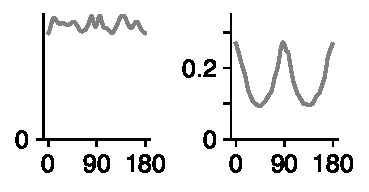
\includegraphics[width=0.4\textwidth]{figures/RunSynthetic_FreePrior_CosineLoss_OnSim_VIZ_OnlyModel_OtherNoiseLevels_Fig2.py_SimulateSynthetic_Parameterized_OtherNoiseLevels_Grid_VarySize.py_180_2_5_N10000_UNIFORM_STEEPPERIODIC.txt_2_0_10.0_180.pdf}};
  \node[rotate=90, right=0.1cm of plot-10000.west, xshift=-0.5cm, yshift=-0.1cm](prob-label-10000){\ \ probability};
\node[above=0.2cm of temp3, anchor=center] (temp3-1) {};
\node[left=2.8cm of temp3-1, anchor=center](prob-label-d){\Large d};

\node[right=4cm of label-10000.east, anchor=center] (label-40000) {\large N=40,000};
\node[below=0.4cm of label-40000, anchor=center] (temp4) {};
\node[left=1.3cm of temp4, anchor=center] (prior-40000) {\large prior};
\node[right=2.1cm of prior-40000, anchor=center] (resources-40000) {\large resources};
\node[below=0.5cm of label-40000, anchor=north, xshift=-0.1cm] (plot-40000)
  {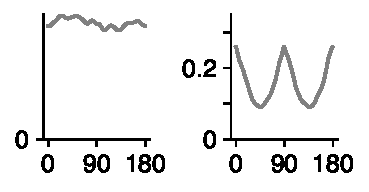
\includegraphics[width=0.4\textwidth]{figures/RunSynthetic_FreePrior_CosineLoss_OnSim_VIZ_OnlyModel_OtherNoiseLevels_Fig2.py_SimulateSynthetic_Parameterized_OtherNoiseLevels_Grid_VarySize.py_180_2_5_N40000_UNIFORM_STEEPPERIODIC.txt_2_0_10.0_180.pdf}};
%  \node[rotate=90, right=0.1cm of plot-40000.west, xshift=-0.5cm, yshift=-0.1cm](prob-label-40000){probability};
\node[above=0.2cm of temp4, anchor=center] (temp4-1) {};
\node[left=2.4cm of temp4-1, anchor=center](prob-label-e){\Large e};

\end{tikzpicture}
\end{document}
